\chapter{Recovering signal event topology} \label{chp:labelTitle}

The previous chapter described in detail how the individual physics objects can be identified and reconstructed, however, in practice the enormeous amount of proton-proton collisions produced at the LHC and collected by the CMS experiment significantly complicates this matter.
As a result the biggest challenge of any physics analyis is to obtain, besides a succesful object identification, an efficient separation of the event topology of interest from the large bulk of background events.
This can be achieved by developing an effective event selection procedure that excludes events based on specific kinematic requirements, as will be demonstrated clearly in this chapter.
\\
\\
Such an event selection starts off with some basic identification and cleaning conditions and proceeds by fine-tuning the kinematic constraints in order to perfectly match with the analysis-specific requirements. Hence the selected event signatures are sequentially \textbf{narrowed down} until the desired event topology is almost completely retrieved. This chapter will first focus on the general kinematic requirements needed to be fullfilled in order to select semi-leptonically decaying top-quark pair topologies, Section~\ref{sec::MainSelec}, and then discuss in Section~\ref{sec::SpecificSelec} the various additional selection conditions introduced in order to optimise the event reconstruction efficiency in this analysis specifically.

\section{Selecting (clean) $\ttbar$+$\mu$ event topologies}\label{sec::MainSelec}
An important aspect of any physics analysis is to select only the event topologies compatible with the considered decay process and avoid detector noise mimicking the signal signature. 
Therefore a dedicated selection and cleaning procedure is applied by combining the online trigger system with an offline event selection in order to reduce the stored event rate while specifying which type of final state particles should be kept for further analysis.

\subsection{Triggering and cleaning of events}\label{subsec::Trigger}
As was already briefly mentioned in Chapter~\ref{chp:CERN}, CMS possesses a complex trigger system that decides whether the considered event is deemed interesting enough to be stored and processed further.
This trigger system uses an exhaustive list of distinct trigger paths, all designed to single out a specific type of final state signature and thus drastically reduce the event rate.
\\

In this analysis the event topology of interest is that of semi-leptonically ($l$ = $\mu$) decaying top-quark pairs, which can be distinguished rather efficiently from background by demanding a muon to be present in each event. This muon signature is rather distinct and will reduce a large portion of the background which is dominated by low-energetic jet processes.
Therefore the trigger path applied in this thesis only keeps events with at least one \textbf{isolated} muon for which the kinematic requirements fullfill $\pT$ $>$ 24 $\GeV$ and $\vert \eta \vert$ $<$ 2.4.
\\
\textit{Is the cleaning part of the triggering? Or is this a separate thing which has to be applied by hand?}

\subsection{Lepton selection criteria}
Since the applied trigger path is not specifically developed for identifying top-quark pairs decaying semi-leptonically, additional selection criteria are required for the leptons in order to further exclude incorrect event signatures. As a result the kinematic requirements are tightened a bit by requiring: $\pT$ $>$ 26 $\GeV$ and $\vert \eta \vert$ $<$ 2.1.
However, the more important lepton selection criteria necessary to apply are responsible for ensuring that the stored muon is a well-defined one.
\\
These so-called muon identification criteria start from Particle-Flow muons, which have been discussed in Section~\ref{subsec::PF}, and are designed to suppress hadronic punch-throughs, cosmic muons and muons from decays in flight of other particles.
They require the candidate muon to be reconstructed as a global one, and the global-muon track fit, with normalised $\chi^{2}$ $<$ 10, to contain at least one muon chamber hit.
Moreover the muon track should have a minimum of two muon stations with matched segments, contain at least one pixel hit and have more than five tracker layers which have been hit. The latter requirement will guarantee, besides suppressing muons from decays in flight, a good $\pT$ measurement for the muon.
Finally muon candidates not originating from the primary vertex are rejected by limiting both the longitudinal and transverse impact parameter: $\vert d_0 \vert$ $<$ 0.2 and $\vert \Delta z \vert$ $<$ 0.5.

Another important identification criterion is the isolation variable which allows to distinghuish prompt muons with high purity from the ones embedded in jets since it determines the hadronic (what about photon) activity around the muon candidate at the interaction vertex. %in a cone of radius $\Delta R$ = 0.4 around the muon candidate. 
It is defined as the scalar sum of the transverse energy of all the reconstructed particles contained within a cone of radius $\Delta R$ = 0.4, excluding the contribution of the muon itself.
However the large number of additional proton-proton interactions significantly complicates the identification of the interaction vertex requiring a correction variable to be applied in order to ensure a correct treatment of these supplementary interactions. 
For this reason a $\Delta \beta$-corrected isolation variable has been developed, which includes for the charged hadrons (CH) only the partons associated with the primary vertex while for the neutral ones (NH and $\gamma$) the estimated PU contribution is subtracted. This contribution can be calculated by halving the PU contribution for charged particles since jets contain on average twice more charged PF particles than neutral ones~\cite{CHContrVsN}. The formula to determine this $\Delta \beta$-corrected isolation variable is given in Equation (\ref{eq::DeltaBetaIso}) and in this analysis $I_{\textrm{rel}}^{\Delta \beta}$ is required to be smaller than 0.12 in order to guarantee the reconstructed muon is well isolated.
\begin{equation}\label{eq::DeltaBetaIso}
 I_{\textrm{rel}}^{\Delta \beta} = \frac{1}{\pT^{\mu}} \left( \sum_{\textrm{CH}} \pT^{\textrm{CH}} + \max(0, \sum_{\textrm{NH}} \pT^{NH} + \sum_{\gamma} \pT^{\gamma} - 0.5 \sum_{PU} \pT^{PU}) \right)
\end{equation}
\textit{Is it pT or ET?}\\
\textit{Need plots?}\\
\textit{Muon veto discussed?}

\subsection{Jet selection criteria}   %Info on: https://twiki.cern.ch/twiki/bin/view/CMS/TopJMERun1#Jets
With the lepton selection clearly established, the next step consists of applying a similar type of identification and cleaning criteria to the selected events.
The goal here is to drastically reduce the fake, badly reconstructed and noise jets while keeping close to 99 $\%$ of the real jets. These jet identification criteria have been studied in detail on 7 TeV data~\cite{JetId7TeV} (is probably private...), and only minor adaptations have been suggested for the 8 TeV data-taking period.
\\
The jet-identification criteria should be applied on the ParticleFlow jets after the different corrections discussed in Section~\ref{subsec::jetReco}: L1L2L3 correction, charged hadron subtraction (\textbf{Is this discussed in a previous chapter?)} %to remove all contributions from charged pileup 
and jet-energy smearing. These calibrations are needed in order to correct for the small discrepancies observed between data and simulation.
\\
\\
In order to select top-quark pairs decaying semi-leptonically, characterised by a well-isolated lepton and four high-energetic jets, each event has to contain at least four jets fullfilling the requirements: $\pT$ $>$ 30 $\GeV$ and $\vert \eta \vert$ $<$ 2.4.
Since each of these jets have to be well separated from the muon identified in the event, all jets for which the $\Delta R$ based distance is lower than 0.3 will be rejected.
\\
The actual jet-identification criteria look at the distribution of the energy fractions and the composition of the different jet constituents.
They reject the noise jets by constraining the energy fraction carried by the charged electromagnetic PF particles ($f_{CEM}$ $<$ 0.99), the energy fraction carried by the charged PF hadrons ($f_{CH}$ $>$ 0), the energy fraction carried by the neutral electromagnetic PF particles ($f_{NEM}$ $<$ 0.99) and the energy fraction carried by the neutral PF hadrons ($f_{NH}$ $<$ 0.99).
\\
\textit{What about number of constituents and muon fraction ?? (+ what is this fHPD (0.98) and n90Hits in event selection file?)}
\\

Another interesting jet-selection contraint, which will be discussed in more detail in Section~\ref{subsec::BTag}, is the requirement to have some of the jets present in the event to be identified as originating from b-quark decays. Even if most of the backgrounds considered for $\ttbar$ decays can have events containing mulitple jets, the possibility that they are labelled as a b-jet is significantly smaller.

\section{Fine-tuning of the event selection}\label{sec::SpecificSelec}

The event selection constraints discussed in the previous section are kept as general as possible in order to be applicable for numerous analyses examining a similar event topology.
Since these selection criteria are centrally managed, their performance is continiously monitored and changing detector conditions are easily taken into account.
In addition, the various synchronization exercises between the different analyses using the same selection criteria significantly improves the selection efficiency. (\textbf{Be sure this is the case!})
\\

The above-mentioned selection criteria, however, still have to be fine-tuned in order to incorporate the analysis-specific requirements.
The analysis discussed in this thesis actually requires a very stringent event selection mainly motivated by the choice to use a Matrix Element method, see Chapter~\ref{ch::MW}. Such a technique examines each event using the full kinematic information and thus needs a large processing time. Therefore it has been opted to restrict the selected number of events as much as possible to avoid spending computational resources on incorrect event topologies.
\\
\\
Two important background-reduction constraints have been applied, each focussing on a different kinematic property and thus aiming to exclude distinct types of events. 
The first one, which is discussed in Section~\ref{subsec::BTag}, exploits the characteristic signature of semi-leptonical decaying top-quark pair events that two of the jets originate from the decay of a b-quark. The second requirement, Section~\ref{subsec::MassCuts}, focuses more on the kinematic properties of the reconstructed jets by demanding their mass combinations to correspond with expectations.
To finalize, Section~\ref{subsec::DataMC} will give an overview of the applied event selection and will demonstrate the obtained (statistical) agreement between data and simulation (illustrated with a selection of kinematic properties).

\subsection{Background reduction using b-jet identification}\label{subsec::BTag}

Top-quark pair-production events for which one of the W-bosons decays hadronical and the other one leptonical are not merely identifiable by the presence of a muon but also by the presence of two jets originating from the decay of the b-quarks.
Exploiting this latter property is an effective manner of distinguishing the event topology from the background, since the decay of the b-quarks has the peculiar feature that it gives rise to a displaced vertex. This because the relatively long lifetime of the b-quark implies that the decay does not occur at the interaction vertex; for more detail see Section~\ref{subsec::jetReco}.
\\ 

In this analysis b-jet identification plays a crucial role in reducing the background contribution since only events with two jets identified as b-jets will be considered. The main background samples for semi-leptonical decaying top-quark events might have events with one jet fullfilling this condition, having two  is less likely (\textbf{Possible to give percentages?}). Hence the considered background samples; W-boson production in association with jets (W+jets), Z-boson production in association with jets (Z+jets) and single-top production in the t-, tW- and s-channel; will almost be completely negligible after applying this b-tagging requirement.
%(\textit{Check if this is also in someway the case when only a double light is applied! .. Yes, main background of W+jets is only 10 $\%$ of ttbar sample! (Total is 20$\%$ of ttbar)})
\\

The b-jet identification algorithms developed by the CMS collaboration are recommended to only be deployed at specific working points, defined as \textit{Loose}, \textit{Medium} and \textit{Tight}. 
Here the Combined Secondary Vertex (CSV) b-tagging algorithm has been considered, for which these working points correspond to a discriminant value of 0.244, 0.679 and 0.898; a tagging probability of around 85$\%$, 69$\%$ and 52$\%$; and a misidentification one of 19$\%$, 5$\%$ and 1$\%$; respectively.
The impressive efficiency for this b-jet identification procedure can be understood by looking at the distribution of the CSV discriminant for different jet flavours given in Figure~\ref{fig::CSVDiscr}, allowing for a clear distinction between the b-flavoured and light-flavoured jets.
\begin{figure}[h!t]
 \centering
 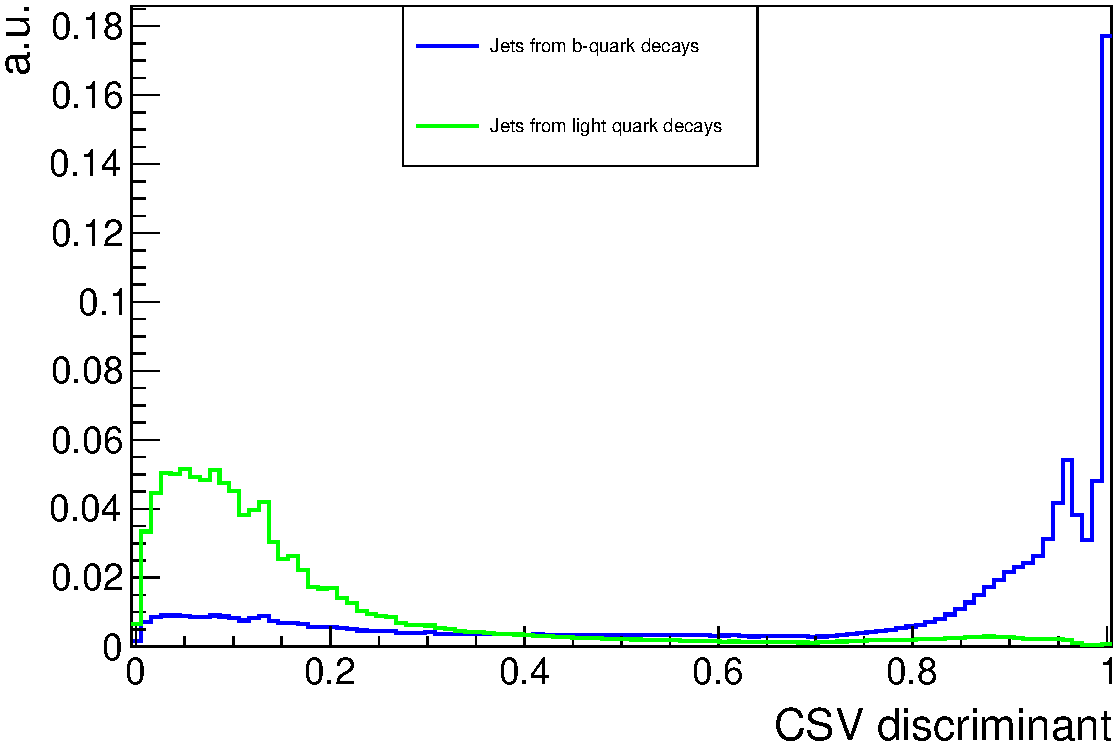
\includegraphics[width = 0.85 \textwidth]{Chapters/Chapter4_EvtSel/Figures/CSVDiscr_LightAndBJets.pdf}
 \caption{Combined Secondary Vertex b-tag discriminant for the different jet-flavours.} \label{fig::CSVDiscr}
\end{figure}

Since in this analysis priority is given to selecting event topologies which closely agree with the expected topology the double Tight CSV b-tagging requirement is expected to be the optimal choice.
This is indeed the case, the fraction of selecting the good jet combination increases from 0.409 up to 0.497 and finally reaches a value of 0.547 when tightening the CSV discriminant value from Loose to Tight. These values have been determined considering simulated semi-leptonic $\ttbar$ events for which information about the corresponding partons is available. (\textbf{Correct this way?})
%This fraction represents the number of events for which all four jets have been assigned to the correct final state particle compared to the number of events with at least one jet reconstructed incorrectly.
%This is indeed retrieved when comparing the number of events for which the four leading $\pT$ jets in the event are correctly picked out from the collection of reconstructed jets for the different b-tag working points. The corresponding fraction of selecting good jet combinations increases from 0.409 up to 0.497 and ends at 0.547 when tightening the CSV discriminant value.
%, which is indeed what can be concluded from Table~\ref{table::bTagResults}.
%This table gives an idea for how many events the four leading $\pT$ jets in the event are correctly picked out from the collection of reconstructed events. This number has been denoted as signal $s$ and will background
%summarizes the number of events for which all four jets are correctly picked out from the collection of reconstructed jets, denoted as signal s, and for which at least one has been wrongly chosen. These two categories, together with the events for which no information about the underlying parton is available, represents the background such that the $s/b$ value gives an idea of the jet reconstruction efficiency for the different b-tag working points.
It has also been investigated whether an improvement could be observed when the CSV discriminant of the light jet candidates is restricted, but since the effect was almost negligible it will not be considered further.
\\

After these double b-tagging requirement the background samples have been significantly reduced and the only remaining contribution comes from the single-top quark events, and then in particular the tW-channel.
This can be understood 
\\
\textit{Now maybe give a Feynman diagram of single top to explain why it remains important.}\\
The application of this double Tight b-tagging algorithm is also the motivation why, besides the background samples discussed before, no other background contributions have been considered for this analysis as they will become completely redundant.
\\

\subsection{Determining the optimal jet combination}
With the b-tag working point and the number of b-tags decided on, the topology reconstruction proceeds by assigning the selected jets to the final state particles expected in semi-muonic $\ttbar$ events.
This reconstruction procedure first identifies the two most energetic jets with sufficiently high CSV-discriminant value and labels all remaining jets as originating from light flavoured partons.
\\
For the two b-jet candidates should then be decided whether they originate from the top quark for which the W-boson decays into two jets, denoted as the hadronical decaying top quark, or from the top quark with the produced W-boson decaying into a muon and corresponding neutrino, the so-called leptonical decaying top quark.
This identification is important since it allows to reduce the number of permutations needed to be considered by the Matrix Element method.
From the collection of light jets only the two expected to originate from the hadronical decaying W-boson have to be identified, but not matched with a specific jet since the up- and down-type jet are difficult to be distinguished. Hence the recovered event topology will have two possible permutations, which both have to be considered.
\\
\\
In this analysis, for which a high reconstruction efficiency is desired, it has been studied whether an improvement can be achieved when the two light-jet candidates are chosen from the three leading $\pT$ jets based on their kinematic resemblance in stead of using the more general approach of merely continuing with the two most energetic light jets.
This light-jet selection is performed simultaneously with the b-jet assignment and is based on a $\chi^{2}$-method using both the invariant mass of the lepton and the b-jet originating from the leptonical decaying top quark, denoted as $M_{lb}$, and the invariant mass of the full hadronic decaying top-quark system, $M_{qqb}$ or $M_{t}$.
\\
The expected values of these invariant masses have been determined by applying a gaussian fit on the distribution obtained for all events passing the above-mentioned event selection requirements, resulting in $\hat{M}_{lb}$ =  107.79 $\pm$ 32.24 $\GeV$ and $\hat{M}_{qqb}$ = 175.03 $\pm$ 17.06 $\GeV$.
The benefit of using the $M_{lb}$ variable in stead of determining the invariant mass of the full leptonic decaying top-quark system is that the reconstruction of the neutrino can be avoided.
A small downside is the non-Gaussian behaviour of this invariant mass distribution such that the fit had to be carefully applied onto a limited range of the distribution.
The obtained invariant mass distributions together with the Gaussian fit function are both given in Figure~\ref{fig::InvMasses}, from which the difference in shape is clearly visible.
\\
\begin{figure}[h!t]
 \centering
 
\includegraphics[width = 0.35\textwidth]{image.png} %Mlb here
 
\includegraphics[width = 0.35\textwidth]{image.png} %Mqqb here
 \caption{Distribution of the invariant masses, $M_{lb}$ on the left and $M_{qqb}$ on the right, together with the applied Gaussian fit function.} \label{fig::InvMasses}
\end{figure}

In this analysis the most plausible jet assignment for the b-jets and the light jets is determined with the same $\chi^{2}$-based procedure for which the formula is given in Equation (\ref{eq::ChiSqMlbMqqb}).
For each event the $\chi^{2}_{i}$ value of the 6 possible jet combinations is calculated and the combination with lowest $\chi^2_{i}$ value is selected.
In case the considered event does not have a third jet present in the event, only the permutation between the hadronic and leptonic b-jet has to be taken into account.
\begin{equation} \label{eq::ChiSqMlbMqqb}
 \chi^{2}_{i} = \frac{(\hat{M}_{lb} - M_{lb,i})^{2}}{\sigma^{2}(\hat{M}_{lb})} + \frac{(\hat{M}_{qqb} - M_{qqb,i})^{2}}{\sigma^{2}(\hat{M}_{qqb})}
\end{equation}

Allowing the third light jet to be part of the chosen jet combination significantly improved the reconstruction efficiency and will therefore be applied in this analysis.
With these extra jet combinations to choose the most plausible one from, the possibility to select the correct two light jets increases from $63.13 \%$ to $76.21 \%$.
Due to this more correct determination of the light jet candidates the overall fraction of selecting good events, mentioned earlier to be 0.547, has improved to $0.666$.
This positive influence can also be seen when comparing the two distributions given in Figure~\ref{fig::ChiSq_4vs5Jets}. 
Here the left-handed distribution contains the $\chi^{2}$ distribution for the chosen jet combination with and without the inclusion of this third jet, while the right-handed one shows the difference in shape of this $\chi^{2}$ distribution (\textit{Shape of a distribution, overkill?}) for the non-chosen jet combinations.
%improvement is also visible from the two $\chi^{2}$ distributions given in Figure~\ref{fig::ChiSq_4vs5Jets}, for which the left-handed one represents the $\chi^{2}$ distribution of the chosen jet combination with and without the inclusion of this third jet while the right-handed one describes the difference in shape of the wrong jet combinations $\chi^{2}$ for the same two options.
\begin{figure}[h!t]
 \centering
 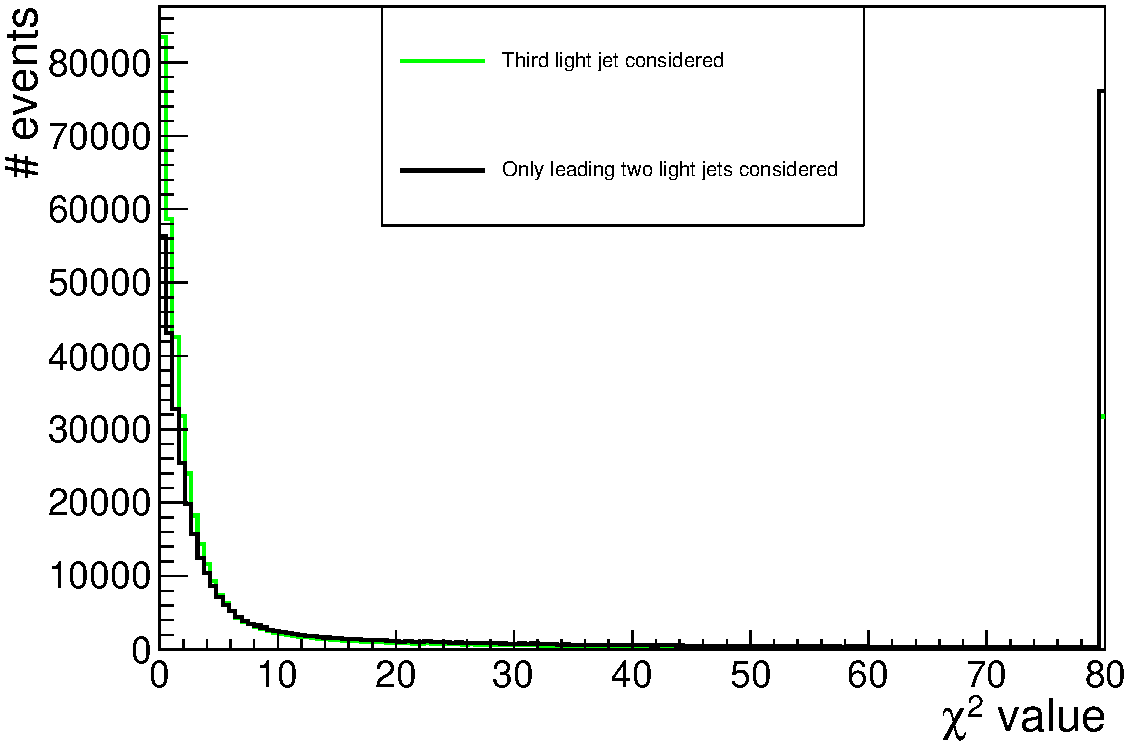
\includegraphics[width = 0.45 \textwidth]{Chapters/Chapter4_EvtSel/Figures/ChosenChiSqDistr_4vs5Jets.pdf}
 
\includegraphics[width = 0.35 \textwidth]{image.png}    %Put here the same but for wrong chisqs (normalised to have comparable numbers!) 
 \caption{... can maybe also plot the normalised shape of the wrong combinations ... (better than the log) + cut on 50 (not 80) -- need solid and dashed line!!} \label{fig::ChiSq_4vs5Jets}
\end{figure}
%\textit{Possible to find a summarising plot? Apply pileup reweighting on numbers...?}\\
%\textit{Mention the improvement when allowing this third jet, if present.}

\subsection{Improving the jet-assignment choice}\label{subsec::MassCuts}
Even though the application of a b-jet identification algorithm will significantly reduce the different background contributions, the reconstruction efficiency can still be enhanced by excluding events using specific kinematic constraints, as will be demonstrated here.
This follows from the fact that the Matrix Element method treats all events as it were semi-leptonical top-quark pair decays such that a visible amelioration can be achieved when augmenting the possibility of choosing the correct event topology.
\\
The two methods that have been considered in order to improve the jet-assignment probability both rely on invariant mass distributions. %(of the hadronical and leptonical decaying top-quark system.)
At first the hadronical decaying top-quark system is restricted by requiring the reconstructed invariant masses, $M_t$ and $M_W$, to lie within a predefined number of standard deviations from the expectation. Secondly a limitation of the $\chi^{2}$ variable, using information from both top quarks as given in Equation (\ref{eq::ChiSqMlbMqqb}), has been studied.
As these two procedures use an overlapping variable to reject undesired events, the invariant mass $M_{lb}$, a correlation between the two is expected.
This correlation, $\chi^{2}$ and $M_{t}$ on the one hand and $\chi^{2}$ and $M_{W}$ on the other hand, is given in Figure~\ref{fig::2Dexclusion}.

\begin{figure}[h!t]
 \centering
 
\includegraphics[width = 0.35 \textwidth]{image.png} %ChiSq vs numbers of sigma deviation from top-mass here (abs value)
 
\includegraphics[width = 0.35 \textwidth]{image.png} %ChiSq vs numbers of sigma deviation from W-mass here (abs value)
 \caption{SET TITLE} \label{fig::2Dexclusion}
\end{figure}

\textit{Now start with the mass restriction.}
\\

\textit{And then discuss the chi-sq cut.}
\\

----------------------------------------------------------------------------------------------------- \\
The effect of this exclusion constraint will definitely not be as important as the application of the b-tag one, since most events already have a rather small $\chi^{2}$ value, as could be seen from Figure~\ref{fig::ChiSq_4vs5Jets}.
However since events with a relatively high $\chi^{2}$ value are less likely to have the correct event topology identified it remains an efficient method to slightly improve the fraction of good reconstructed events.
\\
The optimal $\chi^{2}$ cut-value has been determined by finding a balance between the improvement of the fracion of good reconstructed events on the one hand and the number of selected events on the other hand. Since the goal of this additional cleaning constraint is to reject events for which the topology reconstruction will not result in the desired one, it has been decided require all events to have $\chi^{2}$ $<$ $10$. This will exclude the tail visible in the $\chi^{2}$ distribution in Figure~\ref{fig::ChiSq_4vs5Jets} without reducing the number of selected events too drastically. Since the events not fullfilling this requirement have only a possibility to select the good events of less than 20 $\%$ (\textbf{recheck!}), this constraint improves the fraction for the selected events from $0.666$ to $0.xxx$.
\\

Another event cleaning possibility which have been studied is restricting the invariant mass of the hadronical top-quark system. This constraint is largely correlated with the previously applied $\chi^{2}$ requirement but still allows to reject a number of events for which the combined jets do not originate for this top quark and thus are not correctly reconstructed semi-leptonic decaying top-quark pairs.
Here the top-quark and W-boson mass will need to be reconstructed for each event and should be within a specific unertainty interval around the expected value, both the mass value and uncertainty have been obtained by fitting the distribution after the full event selection with a gaussian function. The expected mass value for the W-boson is $\hat{m}_{W}$ $=$ $83.62$ $\pm$ $17.06$ $\GeV$, distribution given in Figure~\ref{fig::InvWMass}, while the top-quark mass has already been determined during the $\chi^{2}$-procedure ($\hat{m}_{t}$ = $175.03$ $\pm$ $17.06$ $\GeV$).
\begin{figure}[h!t]
 \centering
 
\includegraphics[width = 0.4 \textwidth]{image.png}  %Put here the MW mass distribution (but do not make it too large ...)
 \caption{TO FILL} \label{fig::InvWMass}
\end{figure}

In order to decide on the benefit of applying this second cleaning constraint, its influence has first been studied prior the the $\chi^{2}$ constraint. Due to the large correspondence between the two cleaning procedures it is important to understand clearly the influence of both constraints separately.
\\
Therefore the effect of restricting both the reconstructed W-boson and top-quark mass to a specific number based on the obtained uncertainty has been studied. The different mass ranges which have been studied lie within a 1 up to 5$\sigma$ deviation interval. Again the same motivation as for the $\chi^{2}$ constraint holds in this case, such that the optimal cut-value has been found to be the 2$\sigma$ interval. For this mass range the number of selected semi-leptontic $\ttbar$ events is halved while the reconstruction fraction is improved up to 0.791. 
\\

With the individual contributions understood and found to be useful enough to be applied, only the effect of combining the two had to be investigated. As expected, the correlation between both constraints is very large but since a very minor improvement could be recovered it has been opted to apply both of them. These last two constraints finalize the overall event selection which will be applied in this analysis and as a result the final event reconstruction efficiency, obtained by comparing the number of correctly reconstructed events to the number of events for which a matching parton could be found, is found to be 55.30$\%$. In addition the background contribution became completely negligible and the obtained agreement between data and simulation will now be discussed in detail.
\\

------------------------------------------------------------------------------------------------------ \\
The effect of these two additional event selection constraints clearly hass less of on impact than the b-jet identification algorithm, but is nonetheless an efficient way to reduce the contribution of poorly reconstructed events.

\subsection{Kinematics of remaining events}\label{subsec::DataMC}
The different event selection constraints previously discussed will all be combined in order to reject the background contribution as much as possibly while still remaining with a decent fraction of well reconstructed events.
Under the influence of these three selection requirements, 2 Tight CSV b-tags, $\chi^{2}$ for jet-combination choice smaller than 10, and reconstructed top-quark and W-boson mass within the $2\sigma$ interval of its expectation, the possibility to reconstruct the complete event topology correctly reaches a value of 55.30 $\%$.
\\
Before the agreement between data and simulated events can be compared, the various correction factors needed to incorporate the minor discrepancies between data and simulation have to be applied for the latter type of events.
Most of these corrections have already been discussed earlier, see Section~\ref{sec::}, and have a relatively small influence: \textit{List the different ones!! + some minor explanation. Most of these have mean of 1!}
\\

The only exception, a calibration with corresponding \textbf{large} scale factor, follows from the choice of using the CSV b-jet identification algorithm while requiring two Tight b-tags.
Detailed studies have proven that the b-jet identification efficiency and the misidentification probability to identify a non-b jet as a b jet is not completely similar in data and simulation. 
Therefore b-tag efficiency scale factors have been determined, depending on the event kinematics, in order to correct for these discrepancies~\cite{BTagSF}.
In the case considered here, a very stringent requirement, this additional correction factor becomes very relevant and significantly influences the overall event scale-factor.
\\
\textit{Now shortly explain what it does!}

\paragraph{Scale factors for b-tag efficiency} \hfill \\

\paragraph{Event count} \hfill \\

\paragraph{Kinematic distributions} \hfill \\

---------------------------------------------------------------------------------------------------------------
\\

%\begin{table}[h!t]
% \centering
% \caption{b-tag efficiency for the different working points of the CSV b-tagger.}
% \begin{tabular}{c|c|c|c|c}
%  b-tag working point 	& b-jet efficiency 	& udscg efficiency 	& c-jet efficiency 	& udsg efficiency 	\\
%  \hline
%  double Loose 	& 83.79 $\%$		& 18.91 $\%$		& 42.44 $\%$ 		& 13.4 $\%$		\\
%  double Medium 	& 68.71 $\%$		& 4.57 $\%$		& 18.88 $\%$		& 1.21 $\%$		\\
%  double Tight 	& 52.11 $\%$ 		& 1.22 $\%$ 		& 5.74 $\%$ 		& 0.16 $\%$ 		\\
% \end{tabular}
%\end{table}

\begin{table}[h!t]
 \centering
 \begin{tabular}{c|c|c|c}
		& $\hat{M_{lb}}$ ($\GeV$) 	& $\hat{M_{qqb}}$ ($\GeV$) 	& $\hat{M_{W}}$ ($\GeV$) 	\\
  \hline
  no b-tag 	& 106.9388 $\pm$ 32.0410 	& 174.5792 $\pm$ 17.5196 	& 83.7810 $\pm$ 10.2311 	\\
  b-tag 	& 107.7945 $\pm$ 32.4255 	& 175.0311 $\pm$ 17.0589 	& 83.6161 $\pm$ 10.2171 	
 \end{tabular}
 \caption{Obtained masses from Gaussian fit on distribution obtained before and after the application of the b-tagging requirement.}
\end{table}

\begin{figure}[h!t]
 \centering
 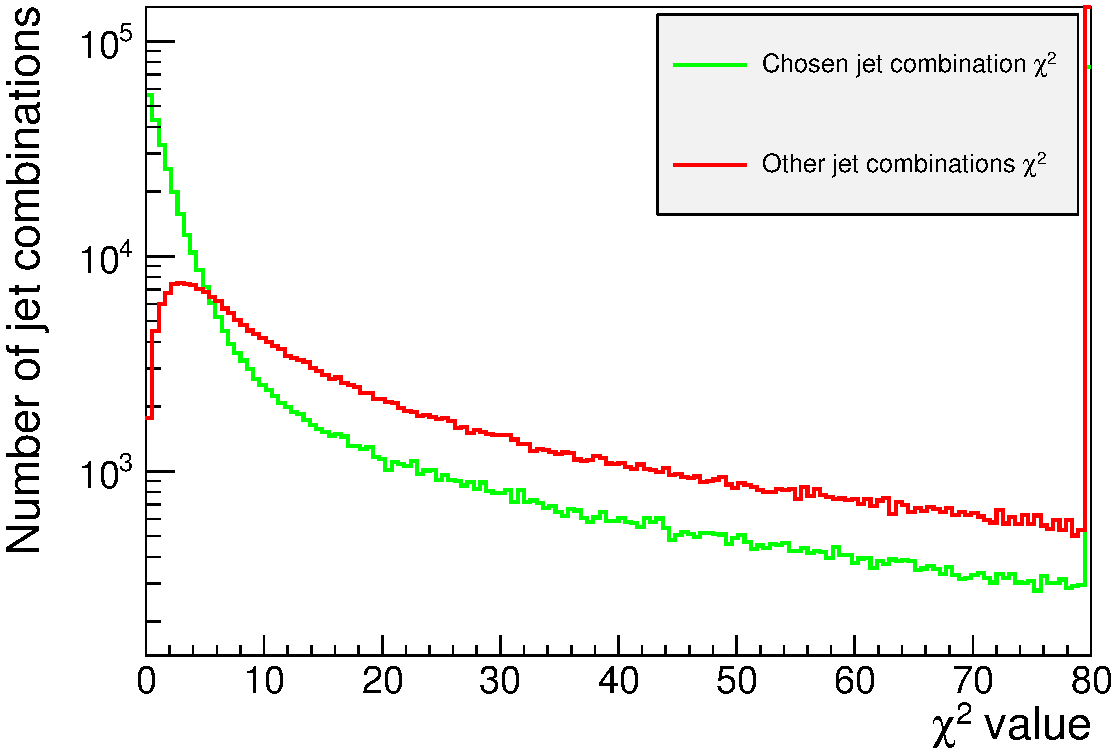
\includegraphics[width = 0.45 \textwidth]{Chapters/Chapter4_EvtSel/Figures/GoodVsBadChiSq_4Jets.pdf}
 %\includegraphics[width = 0.45 \textwidth]{Chapters/Chapter4_EvtSel/Figures/GoodVsBadChiSq.pdf}
 \caption{Difference between good and wrong jet combinations (also create this for 5-jet case). ... Is this in any way relevant??} \label{fig::GoodVsBadChiSq}
\end{figure}

\textit{And will also need to get these numbers for muon channel events alone ... Currently everything is done for muon and electron channel combined!}

